\documentclass[runningheads]{llncs}

% make a proper TOC despite springer's llncs
\setcounter{tocdepth}{2}
\makeatletter
\renewcommand*\l@author[2]{}
\renewcommand*\l@title[2]{}
\makeatletter

\usepackage{ucs}
\usepackage[utf8x]{inputenc}
\usepackage{ngerman}
\usepackage[ngerman]{babel}
\usepackage[T1]{fontenc}
\usepackage[pdftex]{graphicx}
\usepackage[
  pdftex,
  colorlinks=true,
  urlcolor=blue,
  linkcolor=black,
  pdfpagemode=UseNone,
  pdfstartview=FitH,
  pdftitle={Seminar-Ausarbeitung: Web Services},
  pdfauthor={Reinhold Rumberger},
  pdfpagelayout=OneColumn]{hyperref}
\usepackage{array}
\usepackage{tabulary}
\usepackage[refpages,german]{gloss}

\newcommand{\germanquote}[1]{\glqq{}#1\grqq{}}
\newcommand{\decidr}{DecidR}
\newcommand{\anntabwidth}{\textwidth}

\def\gls@section{%
     \section*{\gls@title}%
     \@mkboth{\MakeUppercase\gls@title}{\MakeUppercase\gls@title}%
     \addcontentsline{toc}{section}{\gls@title}}

\author{Reinhold Rumberger}
\tocauthor{\ }
\institute{Institute of Architecture of Application Systems (IAAS),\\
  University of Stuttgart\\
  \email{rumberrd@studi.informatik.uni-stuttgart.de}}
\title{Seminar-Ausarbeitung: Web Services}
\date{27.02.2009}
\makegloss

\begin{document}

  \frontmatter
  \pagestyle{headings}

  \maketitle
  \tableofcontents
  \mainmatter

  \nocite{bk_ralph}

  \titlerunning{Web Services - Einleitung}
  \label{abstract}
  \begin{otherlanguage}{english}
    \begin{abstract}
      Large present-day businesses often use service oriented architectures (SOAs) to implement
      their business processes. One way to implement a SOA is through web services. This paper will
      provide an introduction into the basics of web services. It will then focus on the most
      important technologies used to implement web services in the Java programming environment.
    \end{abstract}
  \end{otherlanguage}


  \label{intro}
  \section{Einleitung}
    In der heutigen Software-Welt wird zunehmend auf Service-Orientierte Architekturen (SOAs)
    gesetzt. Das bedeutet, dass Anwendungen aus einzelnen Diensten aufgebaut werden, die sehr lose
    gekoppelt sind und über eine Art Netzwerk miteinander kommunizieren können. Durch diese
    Eigenschaften lassen sich auf SOA basierende Anwendungen schnell und effizient an neue
    Marktbedingungen anpassen.

    SOAs können durch Web Services implementiert werden. Für Java-Um\-ge\-bung\-en spielen hier vor
    allem JAX-WS 2.0 (Java API for XML-Based Web Services, JSR-224), WS-Metadata 2.0 (JSR-181) und
    JAXB 2.0 (Java Architecture for XML Binding, JSR-222) eine Rolle. Diese Spezifikationen werden
    den Kern der Web Services in \decidr{} bilden.


  \titlerunning{Web Services - SOA}
  \label{soa}
  \section{SOA}
  \nocite{wk_soa}
    Eine \germanquote{SOA} (Service Oriented Architecture) ist eine Software-Architektur, bei der
    lose gekoppelte Dienste miteinander kommunizieren. Die SOA definiert die verfügbaren
    Kommunikationsmethoden und die Methoden zum Auffinden von Diensten. So können verschiedene
    Dienste miteinander verbunden werden, um einen bestimmten Geschäftsprozess zu implementieren.
    Mehrere Dienste werden kombiniert um eine Applikation zu realisieren.

    Die lose Kopplung der Dienste macht die durch sie implementierten Applikationen sehr flexibel.
    So kann relativ schnell auf veränderte Umweltbedingungen reagiert werden. Wenn beispielsweise
    Dienste zufällig aus einer Menge geeigneter Dienste ausgewählt werden, kann man einer
    gesteigerten Nachfrage durch Hinzufügen weiterer Dienste begegnen. Dabei kann es sich sowohl um
    neue Instanzen vorhandener Dienste handeln, als auch um komplett neu entwickelte Dienste, die
    die gleiche Aufgabe erledigen.


  \titlerunning{Web Services - Web Services Grundlagen}
  \label{ws}
  \section{Web Services Grundlagen}
  \nocite{wk_ws}
    Das W3C definiert einen \germanquote{Web Service} folgendermaßen:
    \begin{quote}
      A Web service is a software system designed to support interoperable machine-to-machine interaction
      over a network. It has an interface described in a machine-processable format (specifically
      WSDL). [...]\cite{w3c_wsgloss_ws}
    \end{quote}

    Diese Definition enthält drei Haupteigenschaften von Web Services:
    \begin{description}
      \item[interoperable]
        Web Services sind so ausgelegt, dass sie unabhängig von ihrer Implementierung und der
        Infrastruktur zusammenarbeiten können. Dadurch sind Web Services prinzipiell
        plattformunabhängig, da sie jederzeit auf einer anderen Plattform implementiert werden
        können.
      \item[machine-to-machine interaction]
        Web Services sind nicht designed, um mit Menschen zu interagieren. Jegliche Kommunikation
        über das Netzwerk findet ausschließlich zwischen Web Services statt. Dadurch ist ein aus
        Web Services bestehendes Softwaresystem prinzipiell vollständig automatisiert. Es ist
        selbstverständlich auch möglich, dass ein Web Service Aufgaben an einen Menschen
        weiterleitet und das System so nur teilautomatisiert ist.
      \item[over a network]
        Web Services kommunizieren über ein Netzwerk. Das ermöglicht eine Lastverteilung und den
        zielgerichteten Einsatz spezialisierter Hard- und Software. Es wirft aber auch ein Problem
        auf: Während der Implementierung ist nicht immer bekannt, wo sich der Web Service befinden
        wird. Deshalb existieren Dienste, die eine Liste der bekannten Web Services und ihrer
        Kontaktinformationen bereitstellen.
    \end{description}

    Es gibt zur Zeit zwei relevante Ausprägungen von Web Services: die
    \germanquote{message-oriented Web Services} und die \germanquote{RESTful Web Services}. In der
    Vergangenheit stellten RPC-basierte Web Services die einzige Ausprägung dar. Diese Web Services
    bauten auf \germanquote{remote procedure calls} auf. Heute ist diese Ausprägung nicht mehr
    relevant und wird hier ignoriert.\\
    Es folgt eine kurze Vorstellung der relevanten Ausprägungen:

    \paragraph{RESTful Web Services:}
      Diese Ausprägung orientiert sich stark an HTTP. Deshalb wird die Schnittstelle dieser Sorte
      Web Services auf wenige, von HTTP bereitgestellte, Operationen beschränkt (z.B. GET, PUT und
      DELETE). Durch die Beschränkung der Operationen ist eine bessere Integration mit dem
      HTTP-Protokoll möglich. So kann der Aufwand verringert werden, der für die
      Serialisierung/Deserialisierung von Konstrukten einer Hochsprache in ein XML-Format zu
      transportzwecken nötig ist. Allerdings lassen sich so mit vertretbarem Aufwand nur sehr
      einfache Web Services implementieren. Komplexere Web Services würden einen hohen
      Kommunikations- und Wartungsaufwand erfordern.\\
      Diese Ausprägung ist nicht standardisiert, was dazu führt, dass nicht ganz klar ist, was
      einen RESTful Web Service ausmacht. Somit ist diese Ausprägung für \decidr{}
      uninteressant.\footnote{Diese Darstellung ist stark vereinfacht. Deshalb sind einige der
      Möglichkeiten der RESTful Web Services unterschlagen worden. Da message-oriented Web Services
      für uns wesentlich interessanter sind, ist diese grobe Darstellung jedoch ausreichend. Für
      Interessierte sei auf \cite{paper_pautasso}, Abschnitt 3 verwiesen.}

    \paragraph{message-oriented Web Services:}
      Diese Ausprägung wird auch \germanquote{Big Web Services} genannt. Während RPC-basierte Web
      Services Prozedur-Aufrufe und RESTful Web Services durch MIME identifizierte Objekte über
      HTTP als Kommunikationseinheit verwenden, benutzen message-orientierte Web Services abstrakte
      Nachrichten. Im Gegensatz zu RPC-basierten Web Services können so verschiedene binär
      inkompatible Programmiersprachen verwendet werden. Im Gegensatz zu RESTful Web Services sind
      message-oriented Web Services unabhängig vom Transportprotokoll. Dadurch können sie flexibel
      den Gegebenheiten angepasst werden und es ist möglich, \germanquote{Qualtity of Service}
      (QoS) auch dann zu gewährleisten, wenn die Kommunikationspartner mehrere Netzwerke mit
      verschiedenartiger Infrastruktur trennen. Diese Unterschiede der Infrastruktur können sowohl
      in der verwendeten Hardware als auch im verwendeten Protokollstack liegen.\\
      Da nur eine von der Implementierung unabhängige Schnittstelle veröffentlicht wird, ist eine
      lose Kopplung gegeben. Diese Schnittstelle ist meist in WSDL beschrieben.

    \paragraph{}
    Um die Interoperabilität von Web Services zu verbessern, publiziert das WS-I\cite{wsi_hp}
    sogenannte Profile. Profile bestehen aus definierten Spezifikationen (z.B. SOAP, WSDL) und den
    zugelassenen Versionen (z.B. SOAP 1.2, WSDL 2.0). Hinzu kommen noch zusätzliche Einschränkungen
    (z.B. \germanquote{der SOAP-Body darf nur genau einen Unterknoten haben}), die Unklarheiten der
    Spezifikationen ausräumen. Außerdem publiziert das WS-I Anwendungsfälle und Testwerkzeuge um
    das Deployen profilkonformer Web Services zu erleichtern.\\
    Da diese Profile die Zahl der einsetzbaren Standards stark einschränken, erleichtert die
    Beschränkung auf ein Profil (z.B. das \germanquote{WS-I Basic Profile}) die Implementierung und
    das Deployment erheblich. Existierende Frameworks und IDEs kennen und unterstützen diese
    Profile und können aufgrund der Einschränkungen detailliertere Annahmen machen, was den Einsatz
    von \gloss[nocite]{depl_desc}Deployment Deskriptoren weitgehend überflüssig macht und den
    benötigten Abstraktionsgrad der Laufzeitumgebung erheblich verringert.

    Es gibt desweiteren Standards, die die Fähigkeiten von Web Services erweitern. Diese Standards
    haben meist einen Namen nach dem Schema \germanquote{WS-\texttt{x}} (z.B. WS-Security,
    WS-Transaction). Sie bauen auf den Basis-Standards (SOAP, WSDL, etc.) und aufeinander auf um
    zusätzliche Features wie End-to-End-Verschlüsselung oder Transaktionssicherheit zu
    implementieren. Dieser modulare Aufbau minimiert den Aufwand der nötig ist, um einen Web
    Service mit zusätzlichen Features auszurüsten oder einen Standard gegen einen anderen, besser
    geeigneten auszutauschen.

  \label{soap}
  \subsection{SOAP}
  \nocite{wfm_site}
  \nocite{wk_soap}
    SOAP ist ein Nachrichtenprotokoll, das den Austausch strukturierter Daten zwischen vernetzten
    Web Services erleichtert. Das wird dadurch erreicht, dass das Nachrichtenformat standardisiert
    ist und auf XML aufbaut. SOAP selbst definiert keine Methoden zum Übertragen von Daten;
    stattdessen stützt es sich auf andere Protokolle der Anwendungsschicht (z.B. HTTP, SMTP, FTP)
    für die konkrete Datenübermittlung. Bei der Wahl des Transportprotokolls ist Vorsicht geboten;
    einige Protokolle werden standardmäßig von Firewalls gefiltert und sollten deshalb gemieden
    werden. SOAP stellt die Basis der Kommunikation zwischen Web Services dar.

    Die Wahl von XML als Nachrichtenformat hat sowohl Vor- als auch Nachteile. Positiv sind die
    leichtere Lesbarkeit für Menschen, die bessere Interoperabilität und die vereinfachte
    Fehlersuche. Außerdem sind die Nachrichten validierbar, wodurch Fehler durch ein nicht
    unterstütztes Datenformat ausgeschlossen werden können und bei der Implementierung fehlerhafte
    Datentypen nicht berücksichtigt werden müssen. Dank der Verwendung von XML ist SOAP leicht
    erweiterbar. Allerdings ist XML etwas unhandlich und verlangsamt die
    Verarbeitungsgeschwindigkeit durch seine Verbosität. Dieses Problem kann jedoch mit Binary XML
    und optimierten XML-Parsern minimiert werden.

    Eine minimale SOAP-Nachricht (siehe Abbildung \ref{fig:min_soap}) besteht aus einem
    \texttt{SOAP-\linebreak[0]Envelope}, der einen \texttt{SOAP-\linebreak[0]Header} und einen
    \texttt{SOAP-\linebreak[0]Body} enthält. Während der \texttt{SOAP-\linebreak[0]Body} die
    tatsächliche Nutzlast der Nachricht enthält, stehen im \texttt{SOAP-\linebreak[0]Header}
    Metadaten, die für die Datenverarbeitung und -übertragung wichtige Parameter enthalten.
    Zusätzlich unterstützt SOAP sogenannte \germanquote{Features}, die Einfluss auf die
    Datenverarbeitung und -übertragung nehmen können. Da diese jedoch unter das Thema
    \germanquote{Erweiterbarkeit von SOAP} fallen, sprengen sie den Rahmen dieser Arbeit.

    \begin{figure}[ht!]
      \centering
      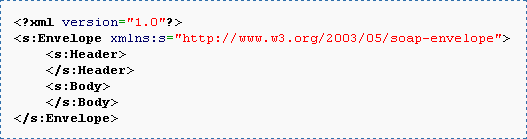
\includegraphics[width=\textwidth]{../images/min_soap.png}
      \caption{Minimale SOAP-Nachricht}
      \label{fig:min_soap}
    \end{figure}


  \subsection{WSDL}
  \label{wsdl}
  \nocite{wk_wsdl}
  \nocite{tut_wsdl}
    An dieser Stelle sei auf den Foliensatz \germanquote{Workflow, Objects and Web
    Ser\-vi\-ces}\cite{wfm_ch7} der Vorlesung \germanquote{Workflow Management}\cite{wfm_site}
    verwiesen. Dort befindet sich wichtige Terminologie, die an dieser Stelle vorausgesetzt wird.

    WSDL (Web Services Description Language) ist eine XML-basierte Sprache zur Beschreibung der
    öffentlichen Schnittstellen von Web Services und ihrer Zugriffsmethoden. Ein WSDL-Dokument ist
    typischerweise mit XML-Schema validierbar. Die wichtigsten Elemente eines WSDL-Dokuments sind:
    \begin{description}
      \item[types]
        Definiert die Datentypen, die in den Messages verwendet werden (siehe Abbildung
        \ref{fig:wsdl_types}). Diese Definition ist abstrakt und unabhängig von der
        Implementierungssprache des Web Service.
      \item[messages]
        Beschreibt die Nachrichten, die ein Web Service akzeptiert und versendet (siehe Abbildung
        \ref{fig:wsdl_messages}). Entspricht den Parametern und dem Rückgabewert in Java.
      \item[portType]
        Beschreibt die verfügbaren Operationen und ihre Messages (siehe Abbildung
        \ref{fig:wsdl_portType}). Eine WSDL-Operation entspricht einer Funktion in klassischen
        Programmiersprachen. Web Services mit dem gleichen portType implementieren per Definition
        die gleiche Funktion.
      \item[binding]
        Definiert das Nachrichtenformat und ein Mapping auf ein Protokoll, das zur Datenübertragung
        verwendet wird (siehe Abbildung \ref{fig:wsdl_binding}). Standard-Bindings sind für SOAP
        über HTTP definiert. Prinzipiell können aber zusätzliche Bindings selbst definiert werden
        oder durch die Laufzeitumgebung bereitgestellt werden.
      \item[service]
        Definiert einen Zugangspunkt für jedes Binding (siehe Abbildung \ref{fig:wsdl_service}).
        Diese Zugangspunkte werden auch \germanquote{Endpoints} genannt. Dieses Element wird meist
        zur Laufzeit generiert und gibt Clients an, wo sie auf den Web Service zugreifen können.
     \end{description}

    Zusätzlich gibt es noch das \texttt{documentation}-Element, das -- ähnlich wie Javadoc für Java
    -- Dokumentation für WSDL-Elemente enthält. Mit dem \texttt{import}-Element aus XML-Schema
    lassen sich Teile eines WSDL-Dokuments auslagern und wiederverwenden. Dafür eignen sich vor
    allem WSDL-Types und WSDL-Messages.

    \begin{figure}[ht!]
      \centering
      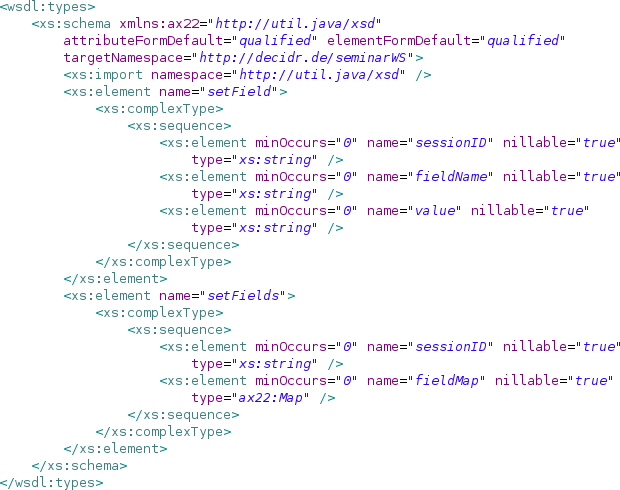
\includegraphics[width=\textwidth]{../images/wsdl_types.png}
      \caption{WSDL-Types}
      \label{fig:wsdl_types}
    \end{figure}

    \begin{figure}[ht!]
      \centering
      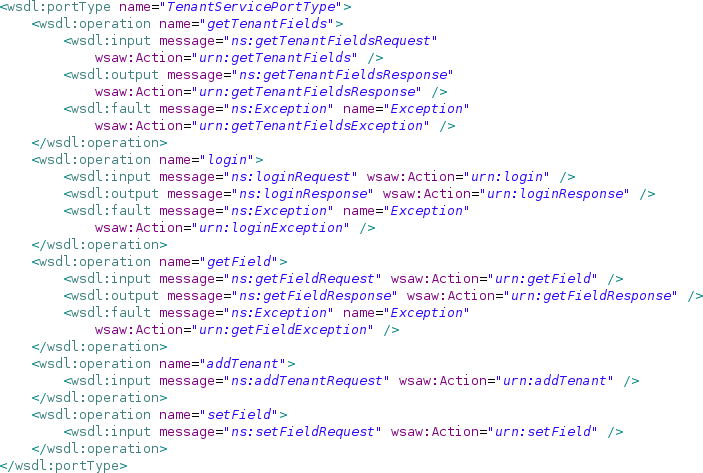
\includegraphics[width=\textwidth]{../images/wsdl_portType.png}
      \caption{WSDL-portType-Element}
      \label{fig:wsdl_portType}
    \end{figure}

    \begin{figure}[ht!]
      \centering
      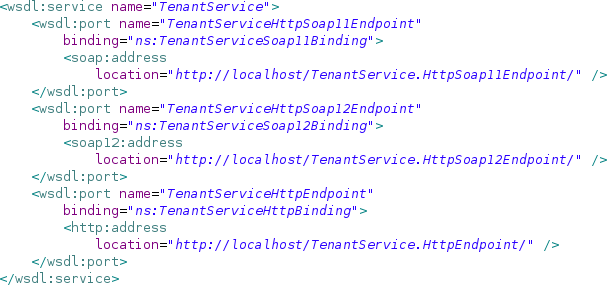
\includegraphics[width=\textwidth]{../images/wsdl_service.png}
      \caption{WSDL-Service-Element}
      \label{fig:wsdl_service}
    \end{figure}

    \begin{figure}[ht!]
      \centering
      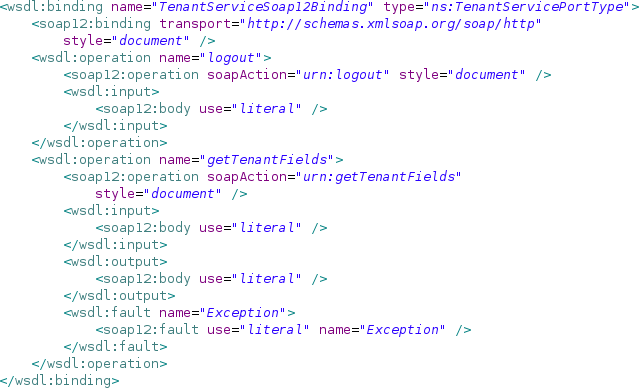
\includegraphics[width=\textwidth]{../images/wsdl_binding.png}
      \caption{WSDL-Binding-Element}
      \label{fig:wsdl_binding}
    \end{figure}

    \begin{figure}[ht!]
      \centering
      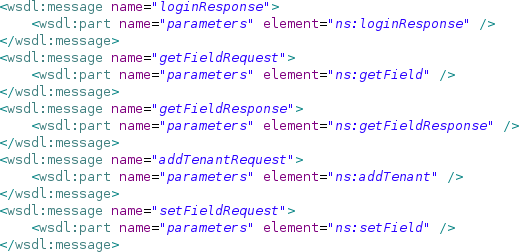
\includegraphics[width=\textwidth]{../images/wsdl_message.png}
      \caption{WSDL-Message-Elemente}
      \label{fig:wsdl_messages}
    \end{figure}

  \label{uddi}
  \subsection{UDDI}
    UDDI\cite{wk_uddi} (Universal Description Discovery and Integration) ist ein Dienst zum
    Auffinden von Web Services in heterogenen Netzwerken. Er hält die WSDL-Beschreibungen und
    einige Metadaten registrierter Web Services bereit. Wegen verschiedener Probleme dieses
    Standards (die den Rahmen dieser Arbeit sprengen) hat er mittlerweile kaum noch Relevanz in der
    Industrie.


  \titlerunning{Web Services - Java und Web Services}
  \label{wsj}
  \section{Java und Web Services}
    \gloss[nocite]{handlers}
    \gloss[nocite]{sei}
    Um in Web Services in Java zu implementieren braucht man vor allem drei Standards: JAX-WS 2.0
    (JSR-224), WS-Metadata 2.0 (JSR-181) und JAXB 2.0 (JSR-222). Diese Standards sind in der Java
    Enterprise Edition 5 enthalten. Somit muss man in dieser Umgebung keine zusätzlichen
    Bibliotheken einbinden. Eine solche JEE-Umgebung stellt Methoden zum veröffentlichen von Web
    Services bereit. Deshalb enthält ein Web Service typischerweise Anwendungslogik, aber keinen
    Code, der direkt mit dem Netzwerk kommuniziert. Das Übersetzen von Java-Objekten in
    XML-Konstrukte (unmarshalling\gloss[nocite]{unmarsh}) und vice versa
    (marshalling\gloss[nocite]{marsh}) übernimmt die Laufzeitumgebung, sofern man dies nicht
    explizit selbst übernimmt.


  \label{jsr224}
  \subsection{JAX-WS 2.0 (JSR-224)}
    Bei JAX-WS\cite{jsr_224} (Java API for XML-Based Web Services) handelt es sich um den
    Nachfolger von JAX-RPC (JSR-101). JAX-RPC war für RPC-orientierte Web Services konzipiert,
    JAX-WS für message-oriented Web Services. JAX-WS enthält alles, was man zum schreiben eines
    einfachen Web Service braucht -- aber keine Methoden um arbiträre Java-Klassen auf XML-Schema
    zu Mappen. Dafür ist JAXB vorgesehen. Außerdem kann man mit JAX-WS kaum Metadaten fürs
    Deployment in die Java-Klassen einbringen. Hier ist die Verwendung von WS-Metadata vorgesehen.

    JAX-WS definiert unter anderem Standard WSDL 1.1 $\Leftrightarrow$ Java Mappings, Standard
    SOAP- und HTTP-Bindings, ein Standard Handler-Framework und vor allem die Client-, Server und
    Core-APIs für JAX-WS-konforme Web Service-Im\-ple\-men\-tier\-ung\-en. Allerdings sind diese
    Standard-Mappings und Standard-Bindings sehr minimalistisch gehalten um Redundanz und
    Überschneidungen mit JAXB und WS-Metadata zu vermeiden.\vfill

    \subsubsection{@WebServiceProvider}\ \\
      \nocite{impl_wsprov}
      Diese Annotation schließt die Verwendung von \texttt{@WebService} aus und kann nur auf
      Klassen angewendet werden, die \texttt{javax.xml.ws.Provider} implementieren. Sie erlaubt den
      direkten Zugriff auf die Empfangene XML-Nachricht. Dadurch entfällt der für das Marshalling
      und Unmarshalling nötige Rechenaufwand. Allerdings muss man bei dieser Methode direkt auf dem
      XML-Baum arbeiten, weshalb sie sich nicht für einfache Web Services eignet. Somit ist diese
      Annotation nur von eingeschränkter Bedeutung für \decidr{}.

      \noindent{}Anwendbar auf:
      \begin{itemize}
       \item Klassen, die \texttt{javax.xml.ws.Provider} implementieren\vfill
      \end{itemize}
      \tymin=75pt
    \begin{tabulary}{\anntabwidth}{|l|L|L|}
    \hline
    \textbf{Parameter} & \textbf{Zweck} & \textbf{Standard} \\
    \hline
      serviceName &
      Wird als \texttt{name}-Attribut im \texttt{wsdl:service}-Element des generierten
      WSDL-\linebreak[0]Dokuments genutzt. &
      \germanquote{} \\
    \hline
      portName &
      Wird als \texttt{name}-Attribut im \texttt{wsdl:port}-Element des generierten
      WSDL-\linebreak[0]Dokuments genutzt. &
      \germanquote{} \\
    \hline
      targetNamespace &
      Wird im generierten WSDL-Dokument als \texttt{targetNamespace} verwendet. &
      \germanquote{} \\
    \hline
      wsdlLocation &
      Eine URL, die auf eine vordefinierte WSDL-Datei zeigt. Die URL relativ oder absolut sein.
      Falls Inkonsistenzen zwischen der Implementierung und dem WSDL-Dokument bestehen, wird zur
      Laufzeit darauf hingewiesen. &
      \germanquote{} \\
    \hline
    \end{tabulary} \vfill
    \tymin=10pt
    \begin{figure}[ht!]
      \centering
      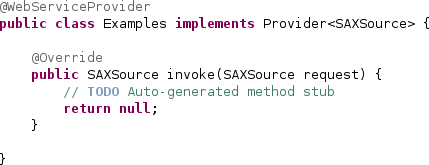
\includegraphics[width=0.9\textwidth]{../images/AtWebServiceProvider.png}
      \caption{Beispiel: @WebServiceProvider}
      \label{fig:wsp}
    \end{figure}

  \label{jsr181}
  \subsection{WS-Metadata 2.0 (JSR-181)}
    WS-Metadata\cite{jsr_181} wurde entwickelt, um die Entwicklung von Web Services zu
    vereinfachen. Deshalb macht WS-Metadata bewusst Annahmen die die Implementierung einiger
    weniger, selten verwendeten Arten von Web Services verhindern.\footnote{Es ist beispielsweise
    möglich einen JAX-WS-konformen Web Service aus den Methoden mehrerer Java-Klassen aufzubauen.
    WS-Metadata nimmt jedoch an, dass jede Klasse genau einen Web Service implementiert und
    umgekehrt.}

    WS-Metadata definiert drei Ansätze für die Entwicklung von Web Services: \germanquote{Start
    with Java}, \germanquote{Start with WSDL} und \germanquote{Start with WSDL and Java}. Der
    letzte Ansatz ist optional und muss von der Laufzeitumgebung nicht unterstützt werden.

    \subsubsection*{Start with Java}
      Bei diesem Ansatz wir zuerst eine Java-Klasse geschrieben, die später als Web Service
      veröffentlicht wird. Wenn die Klasse fertig ist, wird aus ihr mittels
      WS-Metadata-Annotationen ein WSDL-Dokument generiert und veröffentlicht. Das generierte
      WSDL-Dokument folgt standardmäßig den in JAX-WS definierten Java-zu-XML-Mapping.

      Es ist auch möglich den Java-Quelltext aus einem vorher erstellten XML-Schema generieren zu
      lassen.

    \subsubsection*{Start with WSDL}
      Hier wird zuerst aus einem vorher erstellten WSDL-Do\-ku\-ment ein Service Endpoint Interface
      generiert, das dann implementiert wird. Bei der Generierung des SEIs können zusätzlich
      Vorlagen für den Web Service generiert werden, die der Programmierer dann mit der
      Anwendungslogik füllt.

    \subsubsection*{Start with WSDL and Java}
      Hier sind sowohl der Java-Quellcode als auch das WSDL-Dokument vorgegeben. Der Programmierer
      muss lediglich den Java-Quelltext mit den nötigen Annotationen versehen. Leider ist es nicht
      immer möglich existierendem Quellcode auf diese Weise ein WSDL-Dokument zuzuordnen. In diesem
      Fall muss zuerst mit einem der anderen Ansätze eine Wrapper-Klasse erstellt werden, die den
      bestehenden Quellcode mit dem WSDL-Dokument verknüpft.

    \paragraph{}
    Es folgt eine Liste der wichtigsten Annotationen mit ihren wichtigsten Pa\-ra\-me\-tern und
    deren Stan\-dard-\linebreak[0]Wer\-ten. Die Beschreibungen sind gekürzt aus der
    JSR-\linebreak[0]181-\linebreak[0]Spe\-zi\-fi\-ka\-tion\cite{jsr_181} übernommen, weshalb
    teilweise Informationen fehlen. Genauere Details sind in der
    JSR-\linebreak[0]181-\linebreak[0]Spe\-zi\-fi\-ka\-tion\cite{jsr_181} zu finden.\\ \vfill

    \subsubsection{@WebService}\ \\
      Markiert Klassen als Web Services oder Java Interfaces als Service Endpoint Interfaces.

      \noindent{}Anwendbar auf:
      \begin{itemize}
       \item Klassen
       \item Interfaces\vfill
      \end{itemize}
    \begin{tabulary}{\anntabwidth}{|l|L|L|}
    \hline
    \textbf{Parameter} & \textbf{Zweck} & \textbf{Standard} \\
    \hline
      name &
      Wird als \texttt{name}-Attribut im \texttt{wsdl:portType}-Element des generierten
      WSDL-\linebreak[0]Dokuments genutzt. &
      Name der Klasse/\linebreak[0]des Interface \\
    \hline
      serviceName &
      Wird als \texttt{name}-Attribut im \texttt{wsdl:service}-Element des generierten
      WSDL-\linebreak[0]Dokuments genutzt. Darf nicht in SEIs verwendet werden. &
      Name der Klasse + \germanquote{Ser\-vice} \\
    \hline
      portName &
      Wird als \texttt{name}-Attribut im \texttt{wsdl:port}-Element des generierten
      WSDL-\linebreak[0]Dokuments genutzt.\newline Darf nicht in SEIs verwendet werden. &
      \texttt{@WebService.name} + \germanquote{Port} \\
    \hline
      targetNamespace &
      Wird im generierten WSDL-Dokument als \texttt{targetNamespace} verwendet. Für Details bei
      welchen Elementen dieses Attribut gesetzt wird, siehe JSR-181\cite{jsr_181} &
      Im\-ple\-men\-tier\-ungs\-ab\-häng\-ig, siehe JAX-WS\cite{jsr_224}, Abschnitt 3.2 \\
    \hline
      wsdlLocation &
      Eine URL, die auf eine vordefinierte WSDL-Datei zeigt. Die URL kann relativ oder absolut
      sein. Falls Inkonsistenzen zwischen der Implementierung und dem WSDL-Dokument bestehen, wird
      zur Laufzeit darauf hingewiesen. &
      nichts \\
    \hline
      endpointInterface &
      Gibt den Namen des SEIs an, das implementiert werden soll. Das zugehörige Java-Interface muss
      nicht mit \texttt{implements} als implementiert markiert werden. Es bietet sich jedoch an, da
      der Compiler so verifizieren kann, dass das SEI korrekt implementiert wurde.\newline\newline
      Darf nicht in SEIs verwendet werden. &
      nichts\newline \newline Wird bei Bedarf im\-ple\-men\-tier\-ungs\-ab\-häng\-ig generiert,
      wenn es die Zielumgebung erfordert. \\
    \hline
    \end{tabulary} \vfill
    \begin{figure}[ht!]
      \centering
      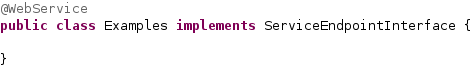
\includegraphics[width=\textwidth]{../images/AtWebService.png}
      \caption{Beispiel: @WebService}
      \label{fig:ws}
    \end{figure} \vfill

    \subsubsection{@WebMethod}\ \\
      Bestimmt ob und unter welchem Namen eine Methode veröffentlicht wird.\footnote{In Axis2 1.4.1
      muss \texttt{operationName} dem Namen der Annotierten Methode entsprechen, da sonst beim
      Aufruf eine \texttt{MedthodNotFoundException} geworfen wird.}

      \noindent{}Anwendbar auf:
      \begin{itemize}
       \item Methoden\vfill
      \end{itemize}
    \tymin=75pt
    \begin{tabulary}{\anntabwidth}{|l|L|L|}
    \hline
    \textbf{Parameter} & \textbf{Zweck} & \textbf{Standard} \\
    \hline
      operationName &
      Wird als \texttt{name}-Attribut des \texttt{wsdl:operation}-Elements genutzt, das der
      annotierten Methode entspricht. &
      Name der annotierten Methode. \\
    \hline
      exclude &
      Dieser Parameter gibt an, dass die annotierte Methode \emph{nicht} veröffentlicht wird.
      \newline Wenn dieser Parameter auf \texttt{true} gesetzt wird, darf \texttt{operationName}
      nicht gesetzt werden. &
      \texttt{false} \\
    \hline
    \end{tabulary} \vfill
    \tymin=10pt
    \begin{figure}[ht!]
      \centering
      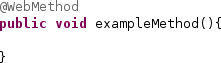
\includegraphics[width=0.5\textwidth]{../images/AtWebMethod.png}
      \caption{Beispiel: @WebMethod}
      \label{fig:wm}
    \end{figure}

    \subsubsection{@Oneway}\ \\
      Eine mit \texttt{@Oneway} annotierte \texttt{@WebMethod} hat keine Output-Message. Das
      bedeutet, dass der Return-Typ \texttt{void} sein muss. Wenn eine mit \texttt{@Oneway}
      annotierte Methode einen Rückgabewert, definierte Exceptions oder \texttt{OUT}- bzw.
      \texttt{INOUT}-Parameter hat, muss spätestens zur Laufzeit ein Fehler gemeldet werden.

      \noindent{}Anwendbar auf:
      \begin{itemize}
       \item Methoden\vfill
      \end{itemize}\vfill
    \begin{figure}[ht!]
      \centering
      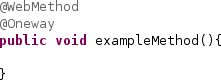
\includegraphics[width=0.5\textwidth]{../images/AtOneway.png}
      \caption{Beispiel: @Oneway}
      \label{fig:oneway}
    \end{figure}

    \subsubsection{@WebParam}\ \\
      Bestimmt die Eigenschaften, mit denen ein Parameter veröffentlicht wird.

      \noindent{}Anwendbar auf:
      \begin{itemize}
       \item Parameter\vfill
      \end{itemize}
    \begin{tabulary}{\anntabwidth}{|l|L|L|}
    \hline
    \textbf{Parameter} & \textbf{Zweck} & \textbf{Standard} \\
    \hline
      name &
      Name des Parameters. Muss in bestimmten Umständen angegeben werden. &
      Normalerweise \texttt{arg\textit{N}}, wobei \texttt{\textit{N}} ein Integer $\geq$ 0 ist. \\
    \hline
      partName &
      Der name des \texttt{wsdl:part}s, das den Parameter repräsentiert. Wird nur in bestimmten
      Umständen benutzt. &
      \texttt{@WebParam.name} \\
    \hline
      targetNamespace &
      Der XML-Namespace des Parameters. Wird nur in bestimmten Umständen benutzt. &
      Entweder der leere Namespace oder der Standard-targetNamespace. \\
    \hline
      mode &
      Gibt an, ob der Parameter als Eingabe, Ausgabe oder beides dient. &
      INOUT, wenn der Parameter von \texttt{javax.xml.ws.Holder<T>} abgeleitet ist, sonst IN. \\
    \hline
      header &
      Wenn der Parameter im Nachrichtenkopf abgelegt ist, \texttt{true}, andernfalls
      \texttt{false}. &
      \texttt{false} \\
    \hline
    \end{tabulary} \vfill
    \begin{figure}[ht!]
      \centering
      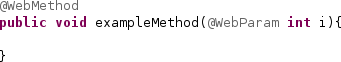
\includegraphics[width=0.8\textwidth]{../images/AtWebParam.png}
      \caption{Beispiel: @WebParam}
      \label{fig:wp}
    \end{figure} \vfill

    \subsubsection{@WebResult}\ \\
      Bestimmt die Eigenschaften, mit denen der Return-Wert einer Methode veröffentlicht wird.

      \noindent{}Anwendbar auf:
      \begin{itemize}
       \item Methoden\vfill
      \end{itemize}
    \begin{tabulary}{\anntabwidth}{|l|L|L|}
    \hline
    \textbf{Parameter} & \textbf{Zweck} & \textbf{Standard} \\
    \hline
      name &
      Name der Ausgabe. Muss unter bestimmten Umständen angegeben werden. &
      Normalerweise \germanquote{return}. \\
    \hline
      partName &
      Der name des \texttt{wsdl:part}s, das die Ausgabe repräsentiert. Wird nur in bestimmten
      Umständen benutzt. &
      \texttt{@WebResult.name} \\
    \hline
      targetNamespace &
      Der XML-Namespace der Ausgabe. Wird nur in bestimmten Umständen benutzt. &
      Entweder der leere Namespace oder der Standard-targetNamespace. \\
    \hline
      header &
      Wenn die Ausgabe im Nachrichtenkopf abgelegt ist, \texttt{true}, andernfalls \texttt{false}.&
      \texttt{false} \\
    \hline
    \end{tabulary} \vfill
    \begin{figure}[ht!]
      \centering
      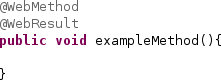
\includegraphics[width=0.5\textwidth]{../images/AtWebResult.png}
      \caption{Beispiel: @WebResult}
      \label{fig:wr}
    \end{figure} \vfill

    \subsubsection{@HandlerChain}\ \\
      Erlaubt es, eine Folge von Handlern für Web Services anzugeben.

      \noindent{}Anwendbar auf:
      \begin{itemize}
       \item Klassen
       \item Methoden
       \item Felder\vfill
      \end{itemize}
    \tymin=75pt
    \tymax=220pt
    \begin{center}
    \begin{tabulary}{\anntabwidth}{|l|L|L|}
    \hline
    \textbf{Parameter} & \textbf{Zweck} & \textbf{Standard} \\
    \hline
      File &
      Referenziert eine Datei, die eine HandlerChain definiert. &
      nichts \\
    \hline
    \end{tabulary}
    \end{center} \vfill
    \tymin=10pt
    \tymax=2\textwidth
    \begin{figure}[ht!]
      \centering
      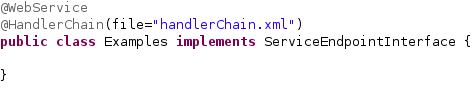
\includegraphics[width=\textwidth]{../images/AtHandlerChain.png}
      \caption{Beispiel: @HandlerChain}
      \label{fig:hc}
    \end{figure} \vfill

    \subsubsection{@SOAPBinding}\ \\
      Spezifiziert, dass der Web Service auf das SOAP-Protokoll gemappt wird. Wird als
      \texttt{@SOAPBinding.Style} \germanquote{DOCUMENT} verwendet, dürfen Klassen und Methoden
      annotiert werden, andernfalls nur Klassen. Methoden, die nicht annotiert sind, verwenden die
      für die Klasse definierten Werte.

      Die Kommunikation zwischen Web Services wird maßgeblich von dieser Annotation geprägt.
      Deshalb sollte man sich detailliert Gedanken machen, welche Werte man hier verwendet. Für
      \decidr{} dürfte die Standardkombination (DOCUMENT, LITERAL, WRAPPED) ausreichen. Für eine
      tiefergehende Diskussion zu diesem Thema siehe \cite{which_wsdl}.

      \noindent{}Anwendbar auf:
      \begin{itemize}
       \item Klassen
       \item Methoden\vfill
      \end{itemize}
    \tymin=75pt
    \begin{tabulary}{\anntabwidth}{|l|L|L|}
    \hline
    \textbf{Parameter} & \textbf{Zweck} & \textbf{Standard} \\
    \hline
      Style &
      Der Kodierungsstil für Nachrichten von und zum Web Service. Entweder \germanquote{DOCUMENT}
      oder \germanquote{RPC}. &
      DOCUMENT \\
    \hline
      Use &
      Der Formattierungsstil für Nachrichten von und zum Web Service. Entweder
      \germanquote{LITERAL} oder \germanquote{ENCODED}. &
      LITERAL \\
    \hline
      parameterStyle &
      Gibt an, ob der SOAP-Body nur die Parameter enthält (\germanquote{BARE}), oder ob sie in ein
      Element eingepackt werden, das nach der Methode benannt ist (\germanquote{WRAPPED}). &
      WRAPPED \\
    \hline
    \end{tabulary} \vfill
    \tymin=10pt
    \begin{figure}[ht!]
      \centering
      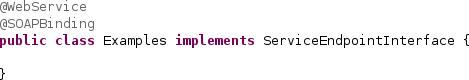
\includegraphics[width=\textwidth]{../images/AtSOAPBinding.png}
      \caption{Beispiel: @SOAPBinding}
      \label{fig:soapb}
    \end{figure} \vfill


  \label{jsr222}
  \subsection{JAXB 2.0 (JSR-222)}
    JAXB\cite{jsr_222} definiert Methoden zum Binding von Java-Klassen auf XML-Schemas und
    umgekehrt. Es erlaubt die Nutzung von Klassen ohne sinnvolles Standard-Binding durch einen Web
    Service. Das Unmarshalling erzeugt XML-Konstrukte, die validiert werden können (z.B. mit JAXP
    1.3).

    Auf der Java-Seite arbeitet JAXB -- ähnlich wie WS-Metadata -- mit Annotationen. Für die
    wichtigsten Annotationen sei auf \cite{ws_crash}, Folie 68 verwiesen.

    Da \decidr{} voraussichtlich vor allem Datentypen verwenden wird, die bereits ein brauchbares
    Standard-Binding aufweisen, wird JAXB in diesem Projekt eine untergeordnete Rolle spielen.

  \label{summary}
  \titlerunning{Zusammenfassung}
  \section{Zusammenfassung}
    Web Services sind ein großes, an Bedeutung gewinnendes Thema, das im Rahmen dieser Arbeit nur oberflächlich behandelt werden kann. Sie werden von großen Unternehmen wie IBM, Microsoft und Google eingesetzt, was sie sehr zukunftssicher macht. Zudem eignen sie sich hervorragend um eine SOA zu implementieren.

    Die für das\decidr{}-Team wichtigste Spezifikation ist WS-Metadata 2.0 (JSR-181)\cite{jsr_181}. Sie definiert und erläutert Annotationen, die jeder in \decidr{} verwendete Web Service benötigt. Da diese Spezifikation die seltene Eigenschaft hat, leicht lesbar zu sein, empfiehlt es sich, einen Blick auf sie zu werfen.


  \newpage
  \titlerunning{Glossar}
  \printgloss{glossary}

  \newpage
  \titlerunning{Literatur}
  \addcontentsline{toc}{section}{Literatur}
  \begin{flushleft}
    \bibliography{literatur}
    \bibliographystyle{splncs}
  \end{flushleft}

\end{document}
